\section{Assignment 7}
\subsection{Feature selection}

Before starting to solve the clusterization problem we decided to do empirical feature selection to get more inpretable and more clear-cut data structure. 
After some attempts we have choosen:
\begin{itemize}
\item
Channel-type nominal features

\begin{itemize}
\item
\texttt{data\_channel\_is\_lifestyle}, \\
\texttt{data\_channel\_is\_entertainment}, \\ 
\texttt{data\_channel\_is\_bus}, \\ 
\texttt{data\_channel\_is\_socmed}, \\
\texttt{data\_channel\_is\_tech}, \\
\texttt{data\_channel\_is\_world} (all are logical).

\item
\texttt{channel} (numeric from 0 to 6)
\end{itemize}
\item
Some words characteristics

\begin{itemize}
\item
\texttt{n\_tokens\_title}, \\
\texttt{n\_tokens\_content}, \\
\texttt{n\_unique\_tokens}, \\
\texttt{average\_token\_length}, \\
\texttt{num\_keywords} (numeric).
\end{itemize}
\end{itemize}

We have also logarithmed all log-normal features.
Unlike previous assignments we haven't deleted zero-length articles to classify them as individual cluster.

\subsection{K-Means Clustering}

First of all we have plotted PCA-plot of our data, you can see the results at Figure \ref{fig:k-means}. One can find 2,7 or some other number of clusters. 

Then we applied built-in function \texttt{kmeans} with parameters $k=3,4,7$ and multi-start with $\texttt{nstart = 100}$, the results of this clusterization are presented at Figure \ref{fig:k-means}.
We should notice that left-bottom cluster in all plots is rather far from the other clusters. During the data analysis we have found out that these points match zero-length articles.  

\begin{figure}[h]
	\centering
	\begin{minipage}[h]{0.49\linewidth}
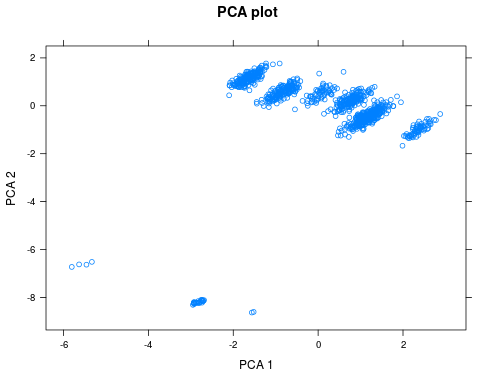
\includegraphics[width=\linewidth]{images/pcaplot_km}
	\end{minipage}
	\hfill
	\begin{minipage}[h]{0.49\linewidth}
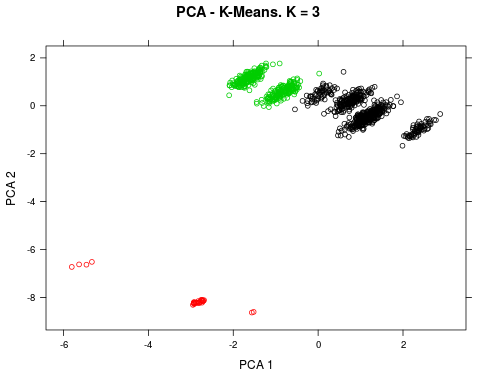
\includegraphics[width=\linewidth]{images/kmean3}
	\end{minipage}
	\begin{minipage}[h]{0.49\linewidth}
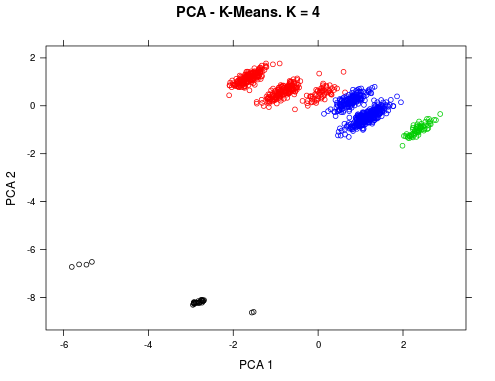
\includegraphics[width=\linewidth]{images/kmean4}
	\end{minipage}
	\hfill
	\begin{minipage}[h]{0.49\linewidth}
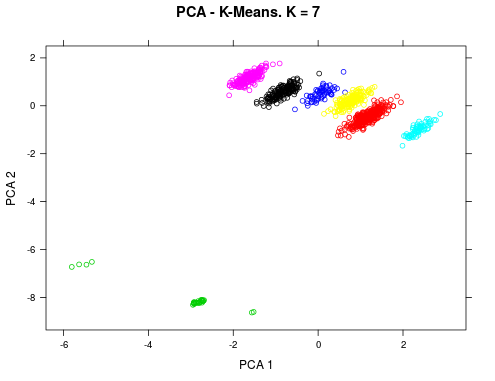
\includegraphics[width=\linewidth]{images/kmean7}
	\end{minipage}
	\caption{PCA plot without clusterization (a), with k-means clusterization with $k=3,4,7$}
	\label{fig:k-means}
\end{figure} 

As we know, k-means method is minimizing the value of total within-cluster sum of squares distance to cluster mean. 
In order to find the optimum number of clusters, we have built plot 
`total within-cluster sum of squares' to `number of clusters' (see Figure {\ref{fig:totalwithin-to-k}).

\begin{figure}[h]
	\centering
	\begin{minipage}[h]{0.49\linewidth}
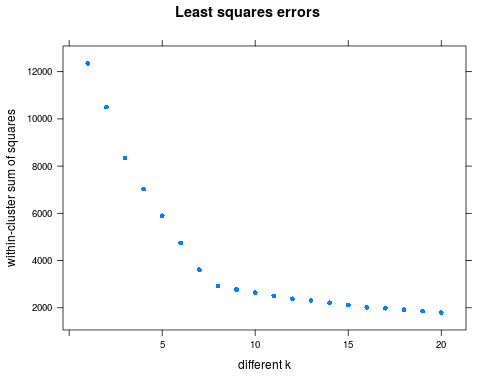
\includegraphics[width=\linewidth]{images/totalwithin}
	\end{minipage}
	\caption{Dependence between `total within-cluster sum of squares' and `number of clusters'}
	\label{fig:totalwithin-to-k}	
\end{figure}

As we can see from the plot, the optimal number of clusters is about 7 (or 8, if we want to divide left-bottom cluster into two parts).

\subsection{Nearest Neighbor clustering with MST}
	We will apply the k-nearest neighbourhood method on the same subset of initial data. To do this at first let's construct the Minimum Spanning Tree (aka MST further) of a complete, weighted and undirected graph, where entities of the dataset serve as vertexes. To compute the weight of each edge we found the distance between the every pair of vertexes. MST is presented in Figure \ref{fig:mst_whole}.

\begin{figure}[h]
	\centering
	\begin{minipage}[h]{0.1\linewidth}
\includegraphics[width=\linewidth]{mst_whole.pdf}
	\end{minipage}
	\caption{Minimum Spanning Tree of dataset.}
	\label{fig:mst_whole}	
\end{figure}	
	
	From the resulting MST we will delete $k$ edges with the greatest weights to obtain graph with $k$ strongly connected components, and they form $k$ clusters. How one could see the clustering with $k=7$ is more natural for this example, so we will apply kNN method with $k = 7$ numbers of clusters as parameter. Graph included $7$ connected components and final clustering are presented in Figure \ref{fig:mst_whole_removed_heaviest} and in Figure \ref{fig:mst_clusters_splitted} respectively.

\begin{figure}[h]
	\centering
	\begin{minipage}[h]{0.1\linewidth}
\includegraphics[width=\linewidth]{images/mst_whole_removed_most_heaviest.pdf}
	\end{minipage}
	\caption{Graph of data after removing the $k=7$ heaviest edges from Minimum Spanning Tree.}
	\label{fig:mst_whole_removed_heaviest}	
\end{figure}	

\begin{figure}[h]
	\centering
	\begin{minipage}[h]{0.1\linewidth}
\includegraphics[width=\linewidth]{images/mst_clusters_splitted.pdf}
	\end{minipage}
	\caption{Clustering via k-Nearest Neighbourhood method with Minimum Spanning Tree.}
	\label{fig:mst_clusters_splitted}	
\end{figure}	

	To compare both method we will use mean the Silhouette Coefficient, which is calculated as $\frac{(b - a) }{\max(a, b)}$ where the mean intra-cluster distance (a) and the mean nearest-cluster distance (b) for each sample.  The mean Silhouette Coefficient for K-Means wit $k = 7$ is equal to $0.44$ and for K-Nearest Neighbourhood method is equal to $0.01$. It may be not give enough information, but if compare two values above we can conclude that clustering better via K-Means method. But if we compare the difference of this indexes for each entity in both method, we can obtain that on average the Silhouette Coefficient k-means method is better.
	


